\chapter{Classification}

\section{Choice of attributes for the decision trees}

For the classification task we decide to use the \textit{Random Forest Classifier}, to choose the model iperparameters we have divided before the dataset in training set (\textbf{80\%} of the customers) and test set (the remaining \textbf{20\%} of the customers), then we have executed a grid search over \textbf{8} iperparameters, for a total of \textbf{2304} combinations. In particular we have searched over:

\begin{table}[h]
\centering
\begin{adjustbox}{width=1\textwidth}
\small
\begin{tabular}{lll}
\textbf{Parameter}       & \textbf{Description}    & \textbf{Values} \\ \rowcolor[HTML]{EFEFEF} 
n\_estimators            & The number of trees in the forest                                  & 100                                          \\
bootstrap                & Whether bootstrap samples are used when building trees             & True                                         \\ \rowcolor[HTML]{EFEFEF} 
max\_depth               & The maximum depth of the tree                                      & [6, 14]                                         \\           
max\_features            & The number of features to consider when looking for the best split & [1, \#features]        \\ \rowcolor[HTML]{EFEFEF}
min\_samples\_split      & The minimum number of samples required to split an internal node   & \{10\%, 1\%, 0.1\%\}                                         \\ 
min\_samples\_leaf       & The minimum number of samples required to be at a leaf node        & \{5\%, 0.5\%, 0.05\%\}                   \\ \rowcolor[HTML]{EFEFEF}
criterion                & The function to measure the quality of a split                     & gini, entropy                                        \\ 
class\_weight            & Weights associated with classes                                    & balanced, not balanced                           

\end{tabular}
\end{adjustbox}
\end{table}

\medskip

Then we have executed a \textbf{10-cross validation} over the training set for each combinations in order to find the best models.
In particular we best ones are:

\medskip

\begin{itemize}
  \item \textbf{Model 1}:
  
  Accuracy in validation phase: \textbf{81.48\%} (std: \textbf{0.02})
  
  Parameters: (bootstrap=True, class\_weight=None, criterion='entropy',
            max\_depth=12, max\_features=1, min\_samples\_leaf=0.005, min\_samples\_split=0.01, n\_estimators=100)
            
  \item \textbf{Model 2}:
  
  Accuracy in validation phase:\textbf{81.46\%} (std: \textbf{0.02})

  Parameters: (bootstrap=True, class\_weight=None, criterion='gini',
            max\_depth=11, max\_features=1, min\_samples\_leaf=0.0005, min\_samples\_split=0.01, n\_estimators=100)

\end{itemize}

\medskip

For both of the models the two most important feature are ps-sep and ps-aug, these are a confirmations of the rules seen in the chapter before. In particulare the importance of features are:

\medskip

\begin{table}[h]
\centering
\begin{adjustbox}{width=.3\textwidth}
\small
\begin{tabular}{lll}
\textbf{Attribute}  & \textbf{Model 1} & \textbf{Model 2} \\ \rowcolor[HTML]{EFEFEF} 
 ps-sep             &  \textbf{25.13\%}       & \textbf{52.22\%}        \\
 ps-aug             &  \textbf{16.77\%}       & \textbf{16.16\%}        \\ \rowcolor[HTML]{EFEFEF} 
 ps-jul             &  \textbf{15.06\%}       & {3.38\%}         \\
 ps-may             &  {8.53\%}        & {2.13\%}         \\ \rowcolor[HTML]{EFEFEF} 
 ps-jun             &  {7.70\%}        & {3.54\%}         \\
 ps-apr             &  {6.85\%}        & {2.40\%}         \\ \rowcolor[HTML]{EFEFEF} 
 pa\_mean           &  {8.75\%}        & {5.11\%}         \\
 limit              &  {5.68\%}        & {5.84\%}         \\ \rowcolor[HTML]{EFEFEF} 
 ba\_mean           &  {2.52\%}        & {2.97\%}         \\
 age                &  {1.71\%}        & {3.17\%}         \\ \rowcolor[HTML]{EFEFEF} 
 education          &  {1.40\%}        & {1.37\%}         \\
 sex                &  {0.99\%}        & {0.62\%}         \\ \rowcolor[HTML]{EFEFEF} 
 status             &  {0.84\%}        & {1.03\%}         \\
\end{tabular}
\end{adjustbox}
\end{table}

In both models the attributes related to the status, sex, education and ages have a very low importance (all under the \textbf{3.17\%}). Instead, as said before, the attributes ps-sep and ps-aug have a very importance (in particular in the second model ps-sep have an importance of \textbf{52\%}).

\section{Results validation with test set and discussion of the best model}

We have trained both selected models over the entire training set in order to predict the credit default over the test set. In this way we can evalute the models using records not yet observed.

\medskip

\textbf{Model 1} (Accuracy 0.7986):

\begin{table}[h]
\centering
\begin{adjustbox}{width=.30\textwidth}
\small
\begin{tabular}{llll}
               & \textbf{precision} & \textbf{recall} & \textbf{f1-score} \\ \rowcolor[HTML]{EFEFEF} 
 \textbf{no}   &  $0.81$            & $0.96$          & $0.88$            \\
 \textbf{yes}  &  $0.68$            & $0.26$          & $0.37$            \\ \rowcolor[HTML]{EFEFEF} 
 \textbf{avg}  &  $0.75$            & $0.61$          & $0.63$            \\
\end{tabular}
\end{adjustbox}
\end{table}

\medskip

\textbf{Model 2} (Accuracy 0.8238):

\begin{table}[h]
\centering
\begin{adjustbox}{width=.30\textwidth}
\small
\begin{tabular}{llll}
               & \textbf{precision} & \textbf{recall} & \textbf{f1-score} \\ \rowcolor[HTML]{EFEFEF} 
 \textbf{no}   &  $0.84$            & $0.95$          & $0.89$            \\
 \textbf{yes}  &  $0.70$            & $0.42$          & $0.53$            \\ \rowcolor[HTML]{EFEFEF} 
 \textbf{avg}  &  $0.77$            & $0.69$          & $0.71$            \\
\end{tabular}
\end{adjustbox}
\end{table}


From this results we can see that the second model performe better over the test set, in particular it has a higher results in the recognition of default=\textbf{yes}.

We tried to train again the second model but this time with a max\_depth equals to \textbf{5} (instead of \textbf{11}), and the results are better than expected:

\medskip

\textbf{Model 3} (Accuracy 0.8246):

\begin{table}[h]
\centering
\begin{adjustbox}{width=.30\textwidth}
\small
\begin{tabular}{llll}
               & \textbf{precision} & \textbf{recall} & \textbf{f1-score} \\ \rowcolor[HTML]{EFEFEF} 
 \textbf{no}   &  $0.84$            & $0.95$          & $0.89$            \\
 \textbf{yes}  &  $0.71$            & $0.42$          & $0.53$            \\ \rowcolor[HTML]{EFEFEF} 
 \textbf{avg}  &  $0.78$            & $0.69$          & $0.71$            \\
\end{tabular}
\end{adjustbox}
\end{table}

Halving the height of the model \textbf{2} we obtain a simplier model that slightly improve the recognition default=\textbf{yes}. 

\section{Decision trees interpretation}

We decide to give an interpretation of Model 3 as it is the simplier and the best among the three different models, to interpret the model we draw the first tree limited to the first three levels:

\medskip

  \begin{minipage}[h]{1\textwidth}
\medskip

  \centering
    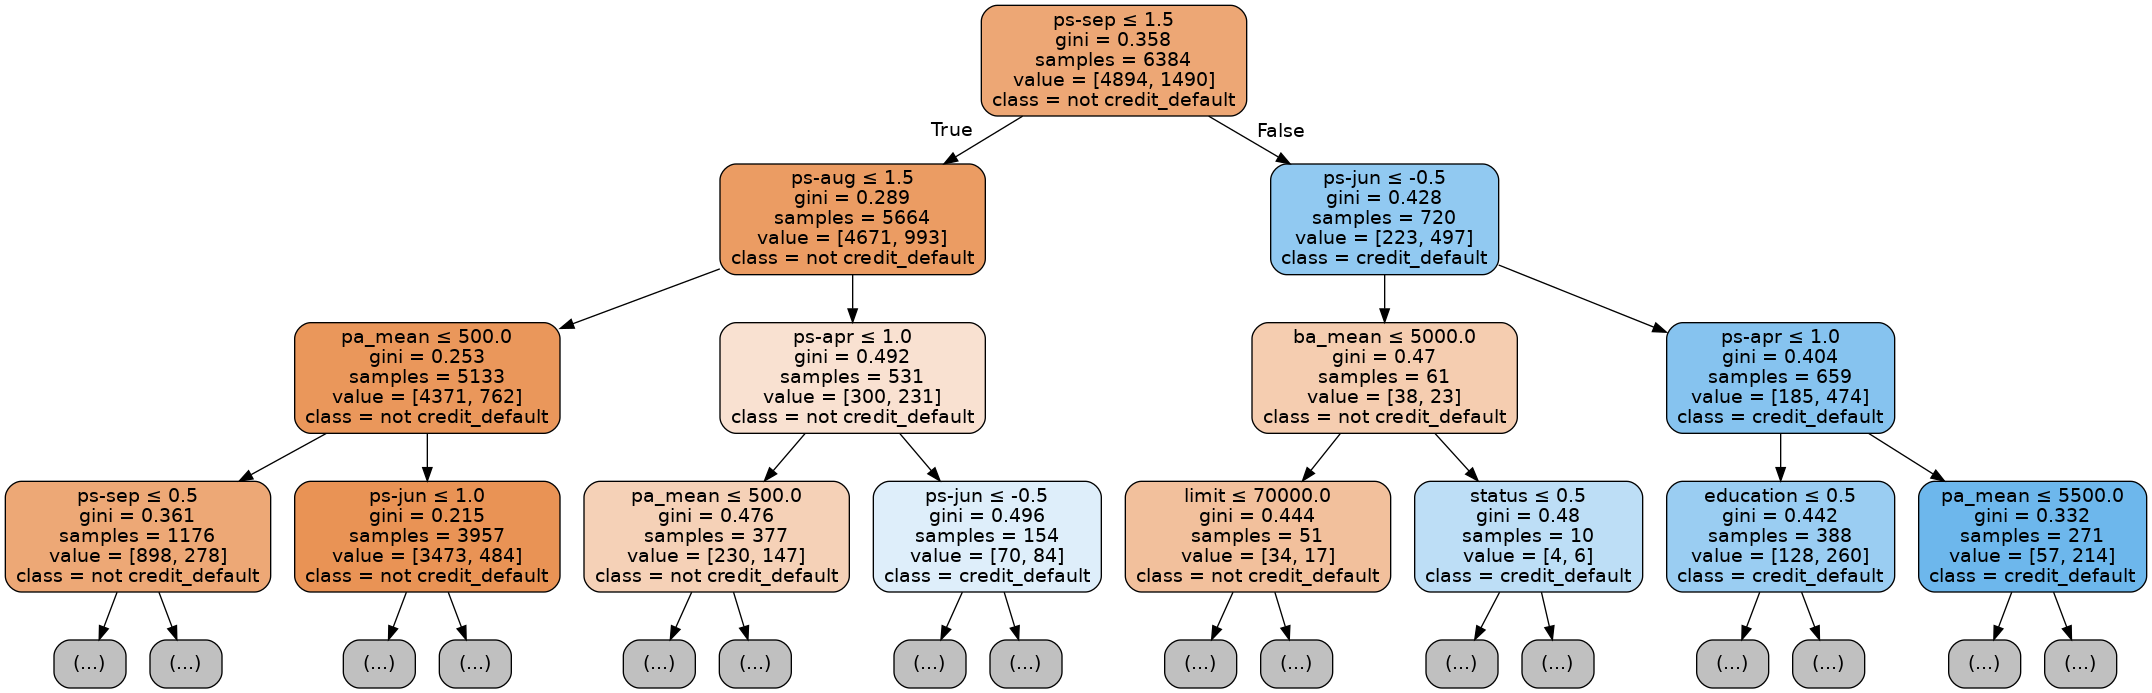
\includegraphics[width=.7\textwidth]{img/ch5/model3}
\medskip

  \end{minipage}

\medskip

From the tree we can see that the first node split the samples in a very unbalanced way (\textbf{88\%} of the customers have a payment status in September equals or less than \textbf{1}). 

\smallskip

If we follow the False branch we are more likely to finish in a default=\textbf{yes} leaf, the only kind of customer with an high payment status in september who don't went in credit default is only the one with a low bill amount mean and a low credit card limit.

\smallskip

On ther other side, the True branch of the first split, we are more likely to finish in a default=\textbf{no} leaf, the only kind of customer in this branch who went in credit default is the one with an high payment status in the month of August, April and June.
